\section{RICH-детектор эксперимента CBM}\label{sec:secCBMrich}

% \textbf{Эта секция пока что выглядит сыровато. Надо смержить с наиболее объёмным вариантом статьи. Надо написать, среди прочего, мотивировку к обеим темам диссера --- ДАК и Билдер! Ещё в секции флес-дак первой части первой главы надо упомянуть, что бестриггерная схема --- это новшество, которое требует испытаний прототипов.}

% \todo \textbf{Может как-то сделать так, чтобы это описание CBM рича было после описания других ричей --- COMPASS, LHCb, HERA-b? Или как раз наоборот, лучше сразу после этой секции?}

% Из диссера Копфера

% For SIS100 the background is already dominated by physical sources like $\gamma$-conversion in the target or $\pi^{0}$-Dalitz decays at a pion suppression factor of $10^3$ (see section 2.6). The electron identification covers the full angular acceptance of the CBM detector, i.e. from \SI{2.5}{\degree} to \SI{25}{\degree} in polar angle and full azimuthal coverage. In order to accommodate the bending of tracks in the dipole magnet, all detectors behind the magnetic field will be wider by a factor 1.5 compared to the height.

Аксептанс детектора, с учётом расширения по горизонтали из-за наличия магнитного поля, разводящего частицы, представляет собой конус \SI{0}{\degree}--\SI{25}{\degree} с вершиной в точке первичного взаимодействия, растянутый по горизонтали в 1.5 раза. Таким образом в плоскости XY угол составляет \SI{0}{\degree}--\SI{37.5}{\degree}.
% Аксептанс детектора составляет $\SI{25}{\degree}$ по вертикали и $\SI{37.5}{\degree}$ по горизонтали.
% Исходя из того факта, что зеркала должны полностью покрывать геометрический аксептанс, ширина детектора выбрана 5268~мм, а высота 4420~мм.

Размер RICH-детектора определяется доступным пространством между кремниевой трековой станцией STS, расположенной внутри магнита, и детектором переходного излучения TRD. С одной стороны, высокая длина радиатора предпочтительна, т.к. она определяет высокий выход черенковских фотонов. С другой стороны, чем меньше расстояние между последней станцией STS и первой станцией TRD, тем выше эффективность трекинга. Из этих соображений для RICH отведено пространство от 1800~мм до 3700~мм по оси пучка, не ограниченное по другим осям ничем, кроме пола. Длина этого пространства вдоль оси пучка составляет 1900~мм. Перед RICH и за ним отведено ещё по 100~мм общего пространства для стыковки магнита, STS, RICH и пучковой трубы. Зеркало расположено на расстоянии 3500~мм от точки взаимодействия, таким образом, рабочая длина радиатора составляет 1700~мм.

% Original English text
% The radiator length is 1.7~m and the volume $\approx 35 m^{3}$. Since the RICH detector will be placed between the STS in the dipole magnet and the TRD detector, its overall length is constrained by the distance between the magnet and its shielding yokes at about 1.6~m from target and the first TRD station. On the one hand, a long radiator is favourable due to the proportionality between photon yield and radiator length according to equation (2.8). On the other hand, a short gap between the tracking detectors STS and TRD is advantageous for tracking which requires a short RICH detector in between. In consequence, the overall length of the RICH detector including radiator, mirror, and support structure is foreseen to be $\approx 2$~m.

% Уменьшение детектора
По причине ограниченного бюджета... \\
Уменьшение детектора означает уменьшение фоточувствительной плоскости, следовательно уменьшение количества МА~ФЭУ, уменьшение площади зеркал, 
Минимизация вклада материала и уменьшение общей стоимости детектора привели к уменьшению детектора.
Так, например, HERA-b RICH (см. секцию~\ref{sec:HerabRich}) регистрирует 33~фотона на кольцо, в то время как в соответствии с моделированием в CBM будет регистрироваться 28~фотонов на кольцо.
Количество зарегистрированных фотонов пропорционально длине радиатора вдоль пучка, а значит уменьшение детектора приводит к понижению его эффективности.

\textbf{ТУТ РАНО ИЛИ ПОЗДНО БУДЕТ КРАСИВАЯ КАРТИНКА}
%\begin{figure}[H]
%\centering
%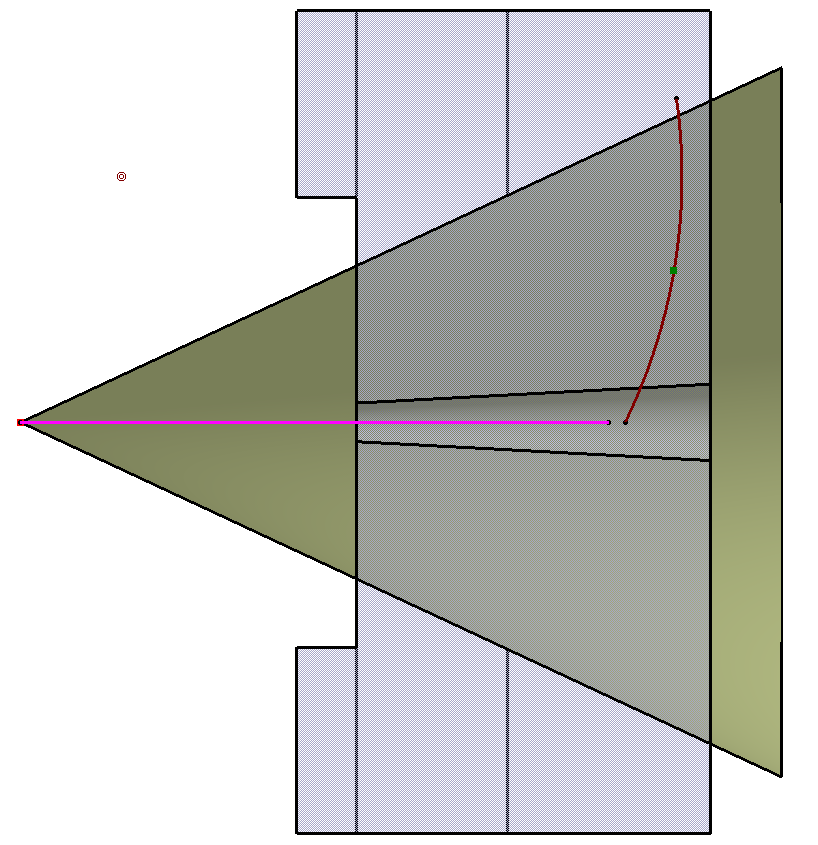
\includegraphics[width=0.7\textwidth]{pictures/RICH_construction.png}
%\caption{Схема детектора CBM RICH, сид сбоку. Жёлтый конус -- геометрический аксептанс.}
%\label{fig:RICHconstruction}
%\end{figure}

% ==============================================================================================
%  ____       _            _                      _                     __   _                _ __  
% |  _ \  ___| |_ ___  ___| |_ ___  _ __      ___| |__   __ _ _ __     / /__| |__   ___  _ __| |\ \ 
% | | | |/ _ \ __/ _ \/ __| __/ _ \| '__|    / __| '_ \ / _` | '__|   | / __| '_ \ / _ \| '__| __| |
% | |_| |  __/ ||  __/ (__| || (_) | |      | (__| | | | (_| | |_     | \__ \ | | | (_) | |  | |_| |
% |____/ \___|\__\___|\___|\__\___/|_|       \___|_| |_|\__,_|_(_)    | |___/_| |_|\___/|_|   \__| |
%                                                                      \_\                      /_/ 
% ==============================================================================================

\subsection{Основные параметры CBM RICH}

28~хитов на кольцо. \\
Средний радиус кольца составляет~4.5~см. \\
Средняя эллиптичность кольца равна~0.937. \\

% ==============================================================================================
%  ____           _ _       _             
% |  _ \ __ _  __| (_) __ _| |_ ___  _ __ 
% | |_) / _` |/ _` | |/ _` | __/ _ \| '__|
% |  _ < (_| | (_| | | (_| | || (_) | |   
% |_| \_\__,_|\__,_|_|\__,_|\__\___/|_|   
%                                         
% ==============================================================================================

\subsection{Радиатор}

% 10 -> нескольких. Почему?!

Разделение электронов и пионов в диапазоне импульсов до нескольких~\GeVoverC{} требует низкого коэффициента преломления радиатора, что определяет выбор углекислого газа в качестве радиатора. $CO_{2}$ имеет пороговый гамма-фактор $\gamma _{th} = 1 / \sqrt{1 - 1/n^{2}} = 33.3$, где $n = 1.00045$ --- коэффициент преломления при нормальных условиях и длине волны 600~нм. Максимальный черенковский угол составляет $\theta = arccos(1/n) = \SI{1.72}{\degree}$. Порог черенковского излучения для заряженных пионов составляет $p = 4.65$~\GeVoverC{}, а для электронов и позитронов --- $p = 0.03$~\GeVoverC{}. При этом порог для каонов составляет $\approx 16$~\GeVoverC{}. Верхняя граница по импульсу составляет $\approx$ 10~\GeVoverC{} и определяется тем, что кольца от электронов и пионов должны быть дискриминированы по радиусу с эффективностью около 90\%.

Нижняя граница длин волн, пропускаемых радиатором, составляет 185~нм. Оценки показывают, что вклад сцинтилляции радиатора в общий счёт фотоэлектронов пренебрежимо мал.

% When designing a RICH detector ``one has to be extremely careful in matching the choice of (gas-)radiator with the sensitive wavelength range of the photon detection system'' [66]. In the case of the CBM-RICH, the low wavelength limit of the photomultiplier sensitivity (see section 3.4) coincides well with the absorption edge of $CO_{2}$ at $\approx 185$ nm (see section 6.2.1).

% \todo остаётся?
% Порог черенковского свечения для пионов составляет $p=4.65$~\GeVoverC{}.

% Т.к. $CO_{2}$ не показывает высокого уровня сцинтилляции его часто добавляют в радиаторы, где другой газ является основным, в качестве гасящего газа. Ожидается около 5~фотонов/МэВ, в основном в синей области спектра. Энерговыделение в радиаторе порядка 1~\GeV{} ожидается при центральном $Au+Au$ столкновении, где рождается $\approx 1000$ минимально ионизирующих частиц, приводящих к $\approx 5000$ сцинтилляционных фотонов, летящих изотропно вдоль трека частицы. Если консервативно предположить, что 20\% фотонов достигает плоскости фотодетекторов и 25\% из них регистрируется, то в результате данного эффекта регистрируется дополнительно около $250$ фотонов, распределённых равномерно. При общем числе каналов порядка 55~000, указанный шум от сцинтилляции добавляет до 0.45\% \todo по всем каналам. Данный показатель находится в допустимом пределе и CBM RICH не теряет в эффективности.

% Due to the fact that $CO_{2}$ does not exhibit a high level of scintillation, it is often added to other radiator gases as quenching gas. Approximately 5 photons/MeV, mostly in the blue wavelength range, are expected [69]. An energy deposit in the radiator of $\approx 1$ GeV{} is expected for a central Au+Au collision with $\approx 1000$ minimum ionizing particles [6] leading to 5000 scintillation photons emitted isotropically along the particle tracks. This leads to $\approx 250$ measured additional photons distributed homogeneously over the photon detector plane when conservatively assuming that 20\% of the photons reach the photon camera with 25\% of them being detected. Given the total of 55 000 channels, noise from scintillation will add up to 0.45\% of all channels. This is well within the noise level that the CBM-RICH detector can tolerate without performance loss [6].

% ==============================================================================================
% __     __                 _ 
% \ \   / /__  ___ ___  ___| |
%  \ \ / / _ \/ __/ __|/ _ \ |
%   \ V /  __/\__ \__ \  __/ |
%    \_/ \___||___/___/\___|_|
%                             
% ==============================================================================================

\subsection{Корпус}

Корпус будет выполнен из алюминия толщиной \todo. Передняя и задняя стенки --- из каптона \todo толщиной \todo.

% ==============================================================================================
%   ____                             _                 
%  / ___| __ _ ___     ___ _   _ ___| |_ ___ _ __ ___  
% | |  _ / _` / __|   / __| | | / __| __/ _ \ '_ ` _ \ 
% | |_| | (_| \__ \   \__ \ |_| \__ \ ||  __/ | | | | |
%  \____|\__,_|___/   |___/\__, |___/\__\___|_| |_| |_|
%                          |___/                       
% ==============================================================================================

\subsection{Газовая система}

% http://hepd.pnpi.spb.ru/hepd/articles/6.pdf
% Я так понял, система для прототипа сопадает с системой для всего детектора.

Закрытая газовая система по мотивам STAR и PHENIX.
Система автоматического регулирования поддерживает $CO_{2}$ при избыточном давлении 2~мбар.
Часть (до 30\%) газа может пропускаться через систему очистки на основе активной меди (active copper puryfier) и осушки (dryer) для избавления от кислорода и влаги.
Система сбора и анализа ``на лету'' следит на попаданием параметров газовой системы в установленные пределы и  запускает необходимые процедуры коррекции в случае выхода за эти пределы.

% ==============================================================================================
%  __  __ _                         
% |  \/  (_)_ __ _ __ ___  _ __ ___ 
% | |\/| | | '__| '__/ _ \| '__/ __|
% | |  | | | |  | | | (_) | |  \__ \
% |_|  |_|_|_|  |_|  \___/|_|  |___/
%                                   
% ==============================================================================================

\subsection{Система фокусировки}

На раннем этапе проектирования CBM RICH исходя из доступного пространства в общей экспериментальной установке было рассчитано, что фокусирующая система CBM RICH должна выполнять одно отражение с помощью двух сферических зеркал радиусом 3~метра, расположенных на расстоянии 3500~мм от точки взаимодействия. Рассматривался также вариант с двойным отражением, при этом вторая группа зеркал была плоская. Зеркала расположены симметрично относительно горизонтальной плоскости, проходящей через ось пучка, и полностью покрывают аксептанс детектора. Площадь каждого зеркала составляет приблизительно 7.5~м$^2$.
Для того чтобы выполнить требование к точности, зеркало такого радиуса технологически возможно изготовить только из сегментов. Рассматривались варианты изготовления различными компаниями. Прототипы тестировались на однородность (\cite{}) и отражательную способность (\cite{}). Зеркала произведённые фирмой Olomuc \todo, были выбраны в качестве зеркал для CBM RICH. Зеркала будут выполнены из SIMAX-стекла толщиной 6~мм и покрыты (отражающим \todo) слоем $Al+MgF_{2}$ с внутренней стороны. Алюминий хорошо отражает фотоны в области видимого всета УФ до 200~нм. Слой $MgF_{2}$ используется как защитный слой с целью предотвращения оксида алюминия, который поглощает ультрафиолет.

% Original English text
% The mirror tiles are made of a 6~mm thick SIMAX glass substrate front-coated with $Al+MgF_{2}$. Aluminium provides a good reflectivity in both the visible and the UV wavelength region down to below 200~nm. The $MgF_{2}$ layer is used as protective layer in order to prevent the formation of UV absorbing aluminium oxide. Mirror tiles from JLO Olomuc were successfully tested in a prototype (see section 5.1), characterised in terms of homogeneity [70] and reflectivity [71], and chosen to be used for the CBM-RICH detector.

Далее рассматривается только одно, верхнее зеркало. Всё описание распространяется и на симметричное нижнее зеркало.

%Основная задача зеркал --- отвести черенковские фотоны в область, где они могут быть зарегистрированы фоточувствительной камерой, которую невозможно расположить напрямую на пути этих фотонов, т.е. в геометрической аксептансе. Это сделает работу последующих детекторов невозможным из-за вторичных частиц.
Основная задача зеркал --- сфокусировать черенковский свет на фоточувствительную камеру. Также присутствет возможность, изменяя угол наклона зеркал, выбирать расположение камеры.

Вообще есть целое направление, в котором люди занимаются тем, что оценивают и обычно стараются минимизировать material budget.

Для того, чтобы фокусировать фотоны на камеру, расположенную за пределами аксептанса, необходимо, чтобы центр сферической поверхности располагался над осью пучка, а сами зеркала полностью покрывали акспетанс. Есть как минимум два варианта геометрии зеркал. В первом зеркало выполняется симметричным относительно горизонтальной плоскости и поворачивается вокруг оси X. При этом возникает зазор между двумя зеркалами, расширяющийся к краям (см. \figref{}), но все зеркала составляются из сегментов двух типов. Более оптимальный способ --- выбрать правильную долю сферы так, чтобы зеркала стыковались без зазора. При этом зеркало получается несимметричным, а следовательно необходимо 4 типа сегментов.

%Данный вопрос также затрагивается в \ref{sec:secMirrorsEvolution}
Ссылка на \figref{fig:MCgeoMirrorsEvolution} и секцию~\ref{sec:secMirrorsEvolution}.

Вот в CBM будет правый вариант. \todo

% Полагая, что пионы и электроны могут быть разделены с эффективностью до 90\% \todo при максимальном черенковском угле $\theta = arccos(1/n)$, 

% The separation of electrons and pions at momenta below 10~\GeVoverC{} requires a low refractive index of the radiator and therefore determines the radiator to be a gas. A $CO_{2}$ radiator is foreseen which has a threshold Lorentz factor of $\gamma _{th} = 1 / \sqrt{1 - 1/n^{2}} = 33.3$, given a refractive index of $n = 1.00045$ at a temperature of \SI{0}{\degreeCelsius}, a pressure of 1000~mbar, and a wavelength of 600~nm. The Cherenkov threshold is $p = 4.65$~\GeVoverC{} for charged pions and $p = 0.03$~\GeVoverC{} for electrons and positrons. The threshold for kaons is $\approx 16$~\GeVoverC{}. The saturated Cherenkov angle for ultrarelativistic particles is $\SI{1.72}{\degree}$. Assuming that pions can be separated from electrons up to 90\% of the maximum Cherenkov opening angle $\theta = arccos(1/n)$, electrons and pions can be separated up to $\approx$ 10~\GeVoverC{} with $CO_{2}$ as radiator gas.

% Явление chromatic absorption в $CO_{2}$ становится заметным только в области длин волн менее 200~нм и, следовательно, не ухудшает разрешения черенковского кольца.

% For $CO_{2}$, chromatic absorption becomes sizeable only in the region below 200 nm (see section 6.2.1) and does not deteriorate the Cherenkov ring resolution significantly as shown below.

% The mirror of the CBM-RICH detector is split into two parts above and below the beam pipe. Each mirror half is oriented towards a photon detection plane and part of a sphere with R = 3.00 m. The total area of the two mirror halves is $12.96 m^2$ . The mirror halves consist of 36 mirror tiles each arranged in four rows of nine tiles. The tiles themselves have a slightly trapezoidal shape in order to minimise gaps in between to 3~mm to~4 mm. Two different tile sizes are foreseen, 430/425.6 mm $\times$ 425~mm for the inner two rows and 425.5/412.5~mm $\times$ 425~mm for the outer rows.

% A tripod concept is foreseen for mounting the mirror tiles on an aluminum frame. Each mirror tile is glued to three actuators allowing for the precise alignment of the tiles in a sphere.

В CBM RICH каждый сегмент зеркал будет крепиться на раме с помощью трёх актуаторов без удалённого управления. Это позволяет корректировать положение отдельных сегментов между запусками пучка. \todo переформулировать
% Ожидается, что нет причин чтобы наклон долей зеркал поплыл после начальной юстировки

В связи с такими-то причинами
, корректируя отклонения от правильного положения, связанные с перемещениями точек механической опоры, находящейся в напряжённо-деформированном состоянии под собственным весом и весом зеркал. Также возможны перемещения в связи с термическим расширением рамы при изменении параметров окружающей среды в экспериментальном зале.

Коллаборациями LHCb и COMPASS разработаны методы \todo, позволяющие выполнять...
Для анализа в моделировании необходимо обеспечить возможность поворота отдельных сегментов зеркал вокруг заданных осей. В связи с этим была построена версия MC-модели, отличающаяся структурой объёмов и обеспечивающая возможность поворота отдельных сегментов зеркал вокруг заданных осей. Эта модель обсуждается в \ref{sec:secRICHgeoMirrorMis}.

Для того чтобы минимизировать рождение вторичных частиц в материале опорных конструкций особое внимание отводится минимизации материала в аксептансе. Исходя из этого опоры зеркал проектируются так чтобы они имели минимальный вес при достаточной жёсткости.
% In order to reduce the production of secondary particles, the material budget of the RICH detector has to be kept low. The mirror support structure is therefore designed as a compromise between stability and light weight.

Сегмент зеркала будет иметь размер около 40см$\times$40см. (точное значение указать невозможно, это ж не прямоугольник)

% ==============================================================================================
%   ____                               
%  / ___|__ _ _ __ ___   ___ _ __ __ _ 
% | |   / _` | '_ ` _ \ / _ \ '__/ _` |
% | |__| (_| | | | | | |  __/ | | (_| |
%  \____\__,_|_| |_| |_|\___|_|  \__,_|
%                                      
% ==============================================================================================

\subsection{Фотодетекторы}

Задача фоточувствительной камеры CBM RICH --- детектировать черенковские фотоны, рождённые заряженными частицами в радиаторе и отражённые от зеркала. Камера разрабатывается для регистрации одиночных фотонов с высокой эффективностью. Для эффективного выполнения реконструкции необходима точная регистрация координат и времени прилёта каждого фотона.
Фоточувствительная камера CBM RICH имеет цилиндрическую форму и состоит из двух половин, расположенных над и под пучком в фокальной плоскости сферических зеркал. Обе половины находятся рядом с дипольным магнитом
% Task of the CBM-RICH photon camera is the detection of Cherenkov photons produced by charged particles in the gas radiator and reflected by the focusing mirror. The camera is developed for the detection of single photons with high efficiency. A precise measurement of position and time of arrival of each photon is required as input for the ring reconstruction algorithm discussed in section 2.5.3.
% The photon camera of the CBM-RICH detector consists of two parts, one above and one below the beam pipe in the focal plane of the spherical mirrors. The two photon detector planes are located in front of the CBM dipole magnet
shielded by the magnet yokes. The Cherenkov rings from the upper mirror half will be projected onto the upper photon detector, rings from the lower mirror half onto the lower photon detector. Each of the two photon detector planes is divided into two parts in order to optimise the angle towards the mirror. Thus, the camera consists of four separated areas, so-called camera modules. Each module covers an area of 0.6~m $\times$ 1.0~m (height $\times$ width). The total active camera area is $2.4 m^{2}$.
The CBM-RICH design foresees the usage of commercially available multianode photomultiplier tubes (MAPMTs) as photon sensors. The use of Micro Channel Plate (MCP) sensors is considered as alternative [6]. Due to the good geometrical coverage of these sensor types, no focusing elements like lenses or Winston cones are envisaged.


Планируется, что фоточувствительная камера CBM RICH будет составлена из модулей, содержащих 2$\times$3 МА~ФЭУ Hamamatsu H12700, см. \figref{fig:H12700drawing}. Один такой МА~ФЭУ имеет габариты 52$\times$52~мм$^2$, между МА~ФЭУ оставляется зазор 1~мм для запаса по точности, таким образом размер модуля составляет 158мм$\times$105мм.

\begin{figure}[H]
\centering
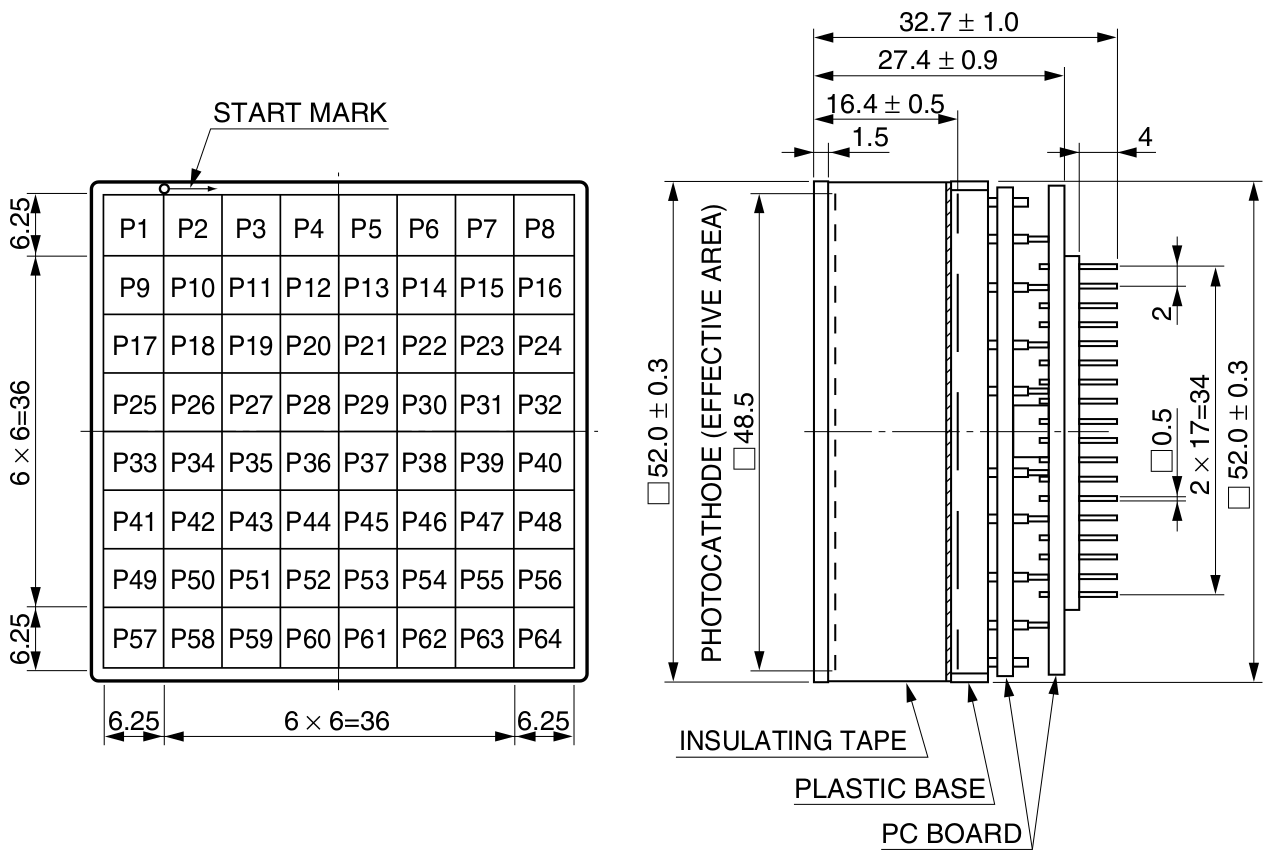
\includegraphics[width=0.7\textwidth]{pictures/H12700_drawing.png}
\caption{Чертёж МА~ФЭУ H12700 из документации.}
\label{fig:H12700drawing}
\end{figure}

В момент написания данной работы ведётся работа по проектированию модуля, разработке программ для FPGA, но имеются изготовленный прототип. Помимо МА~ФЭУ в модуль входят 12~плат передней электроники DIRICH, одна плата, обеспечивающая питание, и одна плата концентрации данных. В основе модуля лежит плата-адаптер, к которой с одной стороны подсоединяются МА~ФЭУ, а с другой --- все платы. CAD-модель и MC-модель модуля показаны на \figref{fig:geoMCmodule}.


% ==============================================================================================
%  __  __                        _   _           __ _      _     _ 
% |  \/  | __ _  __ _ _ __   ___| |_(_) ___     / _(_) ___| | __| |
% | |\/| |/ _` |/ _` | '_ \ / _ \ __| |/ __|   | |_| |/ _ \ |/ _` |
% | |  | | (_| | (_| | | | |  __/ |_| | (__    |  _| |  __/ | (_| |
% |_|  |_|\__,_|\__, |_| |_|\___|\__|_|\___|   |_| |_|\___|_|\__,_|
%               |___/                                              
% ==============================================================================================

\subsection{Магнитное поле в области фоточувствительной камеры}

Моделирование распределения магнитного поля, созданного дипольным магнитом, с помошью пакета TOSCA показало, что фоточувствительная камера расположена в области, где паразитное поле составляет 10--50~мТл. Измерения показали, что для планируемой модели МА~ФЭУ эффективность регистрации одиночных фотонов значительно падает, если поле превышает уровень 1--2~мТл. Таким образом, магнитное поле в области фотосенсоров должно быть опущено до допустимого уровня.

% According to TOSCA 3 calculations, the photon camera is exposed to significant magnetic stray fields in the order of 10~mT to 50~mT. Measurements show that the single photon detection efficiency of the foreseen MAPMTs drops significantly for values exceeding 1~mT to 2~mT especially in the edge and corner pixels [6]. Therefore, the magnetic field strength in the region of the photon sensors has to be kept below this value.

Есть два способа уменьшить поле в области камеры --- повернуть зеркало и, следовательно, отодвинуть камеру от магнита, и поставить магнитный экран вокруг камеры. В CBM RICH была проведена оптимизация угла наклона зеркала точки зрения эффективности реконструкции и было решено спроектировать магнитный экран вокруг камеры.
Есть также третий вариант, который заключается во введении дополнительного отражения на пути черенковских фотонов. Этот подход, однако, был исключён, т.к. дополнительное отражение приводит к увеличению необходимой светочувствительной плоскости, а это значительно увеличивает стоимость детектора.

% In order to cope with the magnetic stray field in the region of the photon camera, two design options are considered and currently studied. The first option is to rotate the two mirror planes and to move the camera modules further away from the beam axis where the magnetic stray field is lower. In addition, a shielding box enfolding the camera modules can reduce the magnetic field strength in the region of the photocathodes significantly. The second option is the use of a second mirror reflecting the Cherenkov photons to the camera positioned farther away from the magnet. This option, however, requires a larger camera surface due to an increased focal length. Details on all design options can be found in [6].

% Ссылка на прогресс репорт 2015 стр. 53.

Положение фоточувствительной камеры в пространстве определяется относительно зеркал исходя из соображений эффективности регистрации колец. В CBM детектор RICH расположен непосредственно за дипольным магнитом, причём отражённые от сферических зеркал черенковские фотоны летят в направлении противоположном пучку. Уменьшение угла наклона зеркал теоретически приводит к повышению эффективности детектора, но на практике невозможно из-за нехватки пространства для размещения камеры в небольшом зазоре между магнитом и конусом аксептанса RICH. Увеличение угла наклона зеркал позволило бы вывести фотодетектор далее вверх из области магнитного поля, но это приводит к нежелательным оптическим эффектам, отрицательно влияющим на эффективность. Следовательно, камера должна быть расположена очень близко к дипольному магниту. Отсюда возникает необходимость экранировать камеру от магнитного поля, составляющего 50-100~мТл в области МА~ФЭУ. Рассчитано, что данное семейство МА~ФЭУ может работать в магнитном поле до 1~мТл без снижения эффективности.

% ==============================================================================================
%  __  __                        _   _                                       
% |  \/  | __ _  __ _ _ __   ___| |_(_) ___     ___  ___ _ __ ___  ___ _ __  
% | |\/| |/ _` |/ _` | '_ \ / _ \ __| |/ __|   / __|/ __| '__/ _ \/ _ \ '_ \ 
% | |  | | (_| | (_| | | | |  __/ |_| | (__    \__ \ (__| | |  __/  __/ | | |
% |_|  |_|\__,_|\__, |_| |_|\___|\__|_|\___|   |___/\___|_|  \___|\___|_| |_|
%               |___/                                                        
% ==============================================================================================

\subsubsection{Магнитный экран вокруг камеры}\label{sec:secCameraShield}

Т.к. рассматривалось два варианта форм фоточувствительной камеры --- четыре плоскости и два цилиндра --- потребовалось прорабатывать два варианта формы магнитного экрана. На \figref{fig:ShieldingBox} показан чертёж первого рассчитанного магнитного экрана для плоского варианта камеры, а на \figref{fig:ShieldingBoxMC} --- первая версия магнитного экрана в CbmRoot.

\begin{figure}[H]
\centering
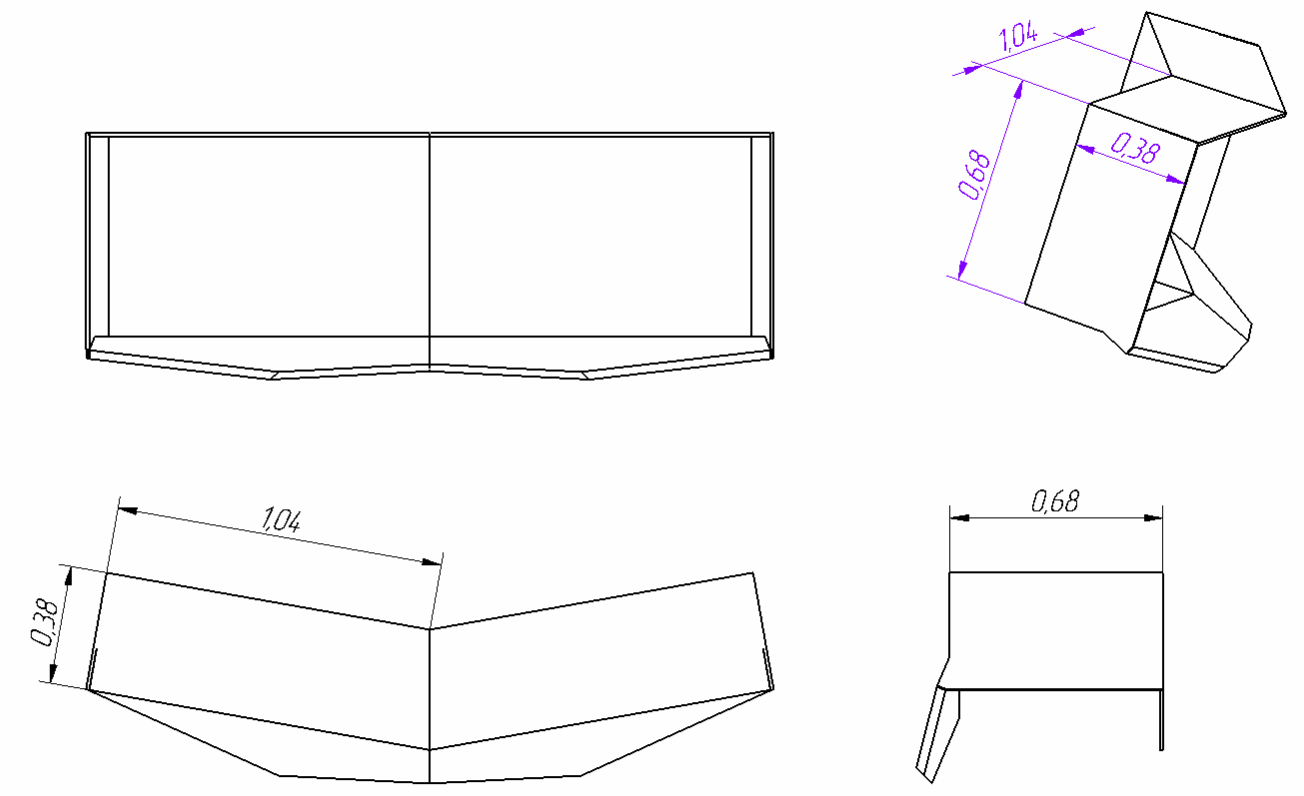
\includegraphics[width=0.7\textwidth]{pictures/First_shielding_box_1.png}
\caption{Первый эскизный проект магнитного экрана.}
\label{fig:ShieldingBox}
\end{figure}

\begin{figure}[H]
\begin{minipage}[b]{0.495\textwidth}
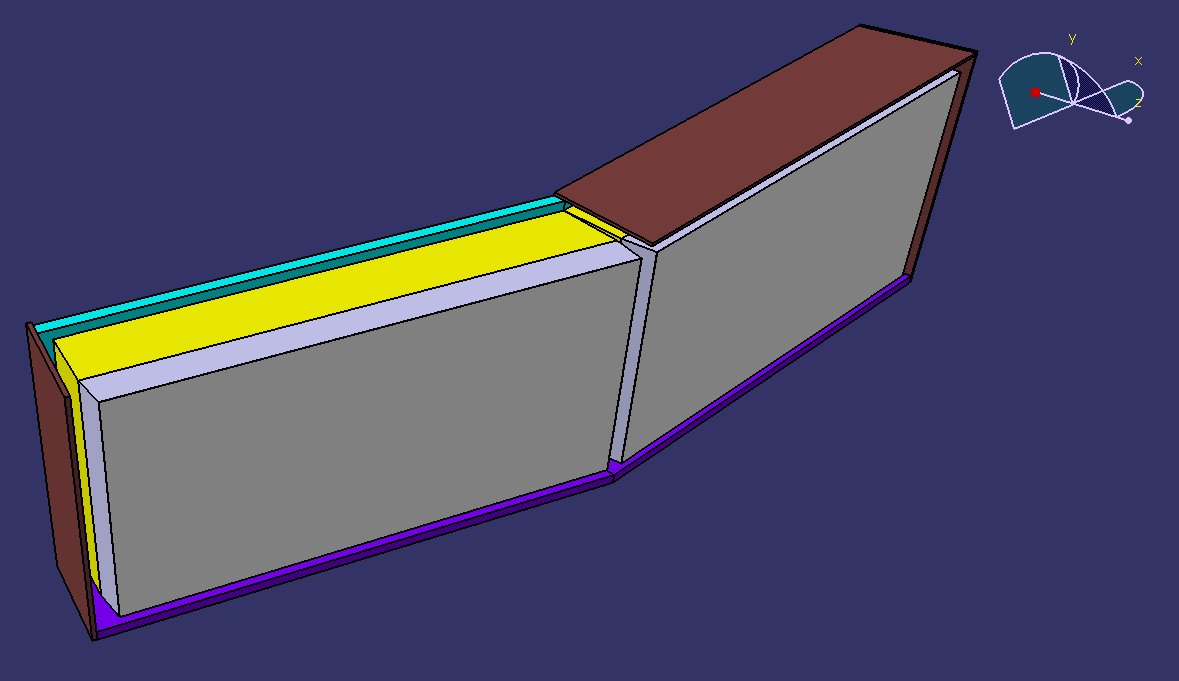
\includegraphics[width=1.0\textwidth]{pictures/ShieldingBox_MC.png}
\end{minipage}
\hspace{0.01\textwidth}
\begin{minipage}[b]{0.495\textwidth}
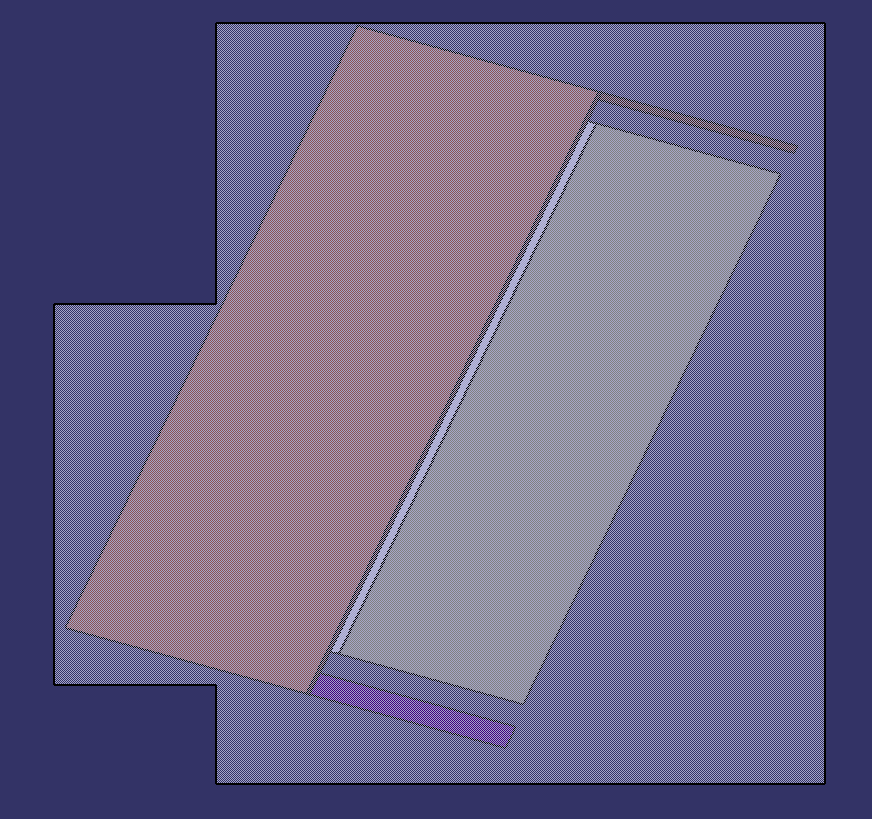
\includegraphics[width=0.7\textwidth]{pictures/ShieldingBox_MC2.png}
\end{minipage}
\caption{Первая версия магнитного экрана в CbmRoot. Серым цветом показаны МА~ФЭУ, жёлтым --- электроника.}
\label{fig:ShieldingBoxMC}
\end{figure}

На момент написания данной работы проект магнитного экрана не был завершён, однако было выполнено эскизное проектирование и моделирование распределения магнитного поля в пакете OPERA (TOSCA) \todo. Было определено, что магнитный экран должен иметь нижнюю и заднюю (ближную к магниту) стенку толщиной 30~мм, а остальные --- толщиной 10~мм. Одной из проблем при проектировании магнитного экрана является задача минимизации массы; т.к. экран должен быть выполнен из материала с высоким коэффициентом магнитной проницаемости, лёгкие металлы типа алюминия не подходят. Масса каждого из двух экранов получилась равна 850~кг. В экране присутствуют отверстия необходимые для отвода кабелей и для обеспечения охлаждения.